%% LyX 2.2.1 created this file.  For more info, see http://www.lyx.org/.
%% Do not edit unless you really know what you are doing.
\documentclass[10pt,english]{article}
\usepackage{helvet}
\usepackage[T1]{fontenc}
\usepackage[latin9]{inputenc}
\usepackage[a4paper]{geometry}
\geometry{verbose,tmargin=1cm,bmargin=1cm,lmargin=1cm,rmargin=2cm}
\pagestyle{plain}
\usepackage{xcolor}
\usepackage{graphicx}

\makeatletter

%%%%%%%%%%%%%%%%%%%%%%%%%%%%%% LyX specific LaTeX commands.
%% Because html converters don't know tabularnewline
\providecommand{\tabularnewline}{\\}

\makeatother

\usepackage{babel}
\begin{document}
\noindent\begin{minipage}[t]{1\linewidth}%
\begin{minipage}[t]{0.65\linewidth}%
\begin{flushleft}
\textbf{\textcolor{teal}{\LARGE{}Curriculum Vitae }}
\par\end{flushleft}{\LARGE \par}
\begin{flushleft}
\textbf{\Large{}}%
\noindent\begin{minipage}[t]{1\columnwidth}%
{\footnotesize{}Title, First Name, Family Name}{\footnotesize \par}

\rule[0.5ex]{0.725\linewidth}{0.02pt}
\begin{flushleft}
\textbf{\large{}Dr. Balakrishna Soorali Ganeshamurthy}
\par\end{flushleft}{\large \par}%
\end{minipage}
\par\end{flushleft}{\Large \par}

\includegraphics[scale=0.02]{pasted1}{\small{}\hspace*{0.3cm}Turnackerstr
19, 70794, Filderstadt, Germany.}{\small \par}

{\small{}
\includegraphics[scale=0.035]{pasted2}\hspace*{0.3cm}balakrishna@web.de}{\small \par}

{\small{}
\includegraphics[scale=0.045]{pasted3}\hspace*{0.3cm}+49
(0) 176-3096-2464}{\small \par}

{\small{}
\includegraphics[scale=0.06]{Birthday_Icon}\hspace*{0.3cm}
21.August.1983}{\small \par}

{\small{}
\includegraphics[scale=0.017]{tls-boca-systems-icon-world-thumb}\hspace*{0.3cm}
Indian}{\small \par}%
\end{minipage}\hspace{1cm}%
\begin{minipage}[t]{0.2725\linewidth}%
\vspace{0.1cm}

\begin{flushright}
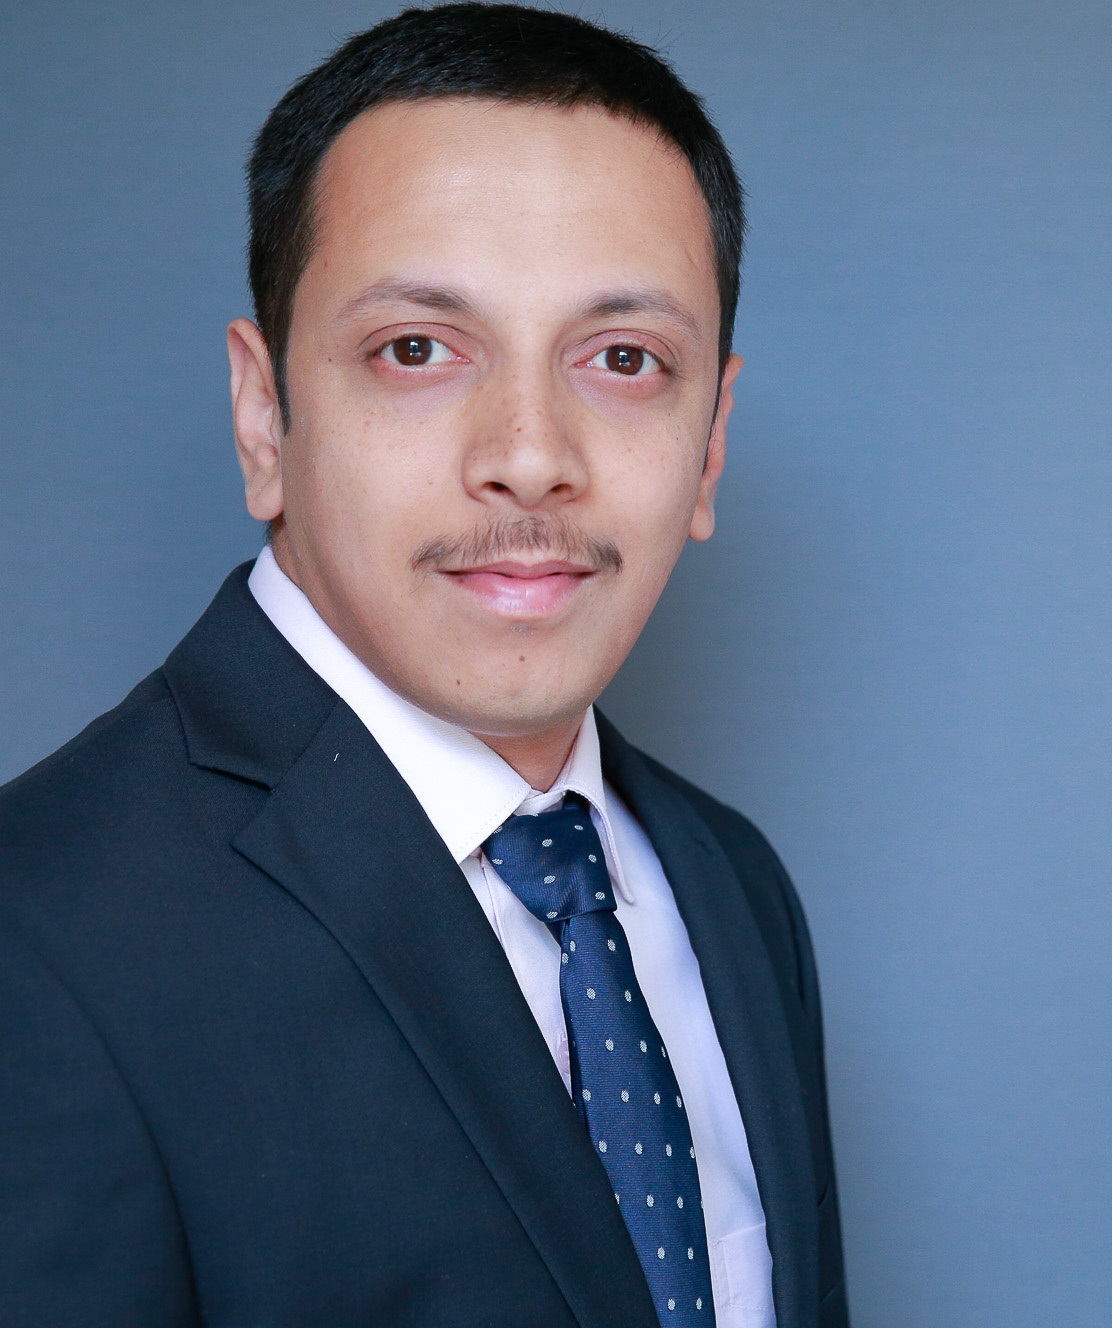
\includegraphics[scale=0.25]{photo}
\par\end{flushright}%
\end{minipage}%
\end{minipage}

\vspace{0.5cm}

\noindent\begin{minipage}[t]{1\columnwidth}%
\textbf{\textcolor{teal}{\large{}Technical Skills :}}{\large \par}

\rule[0.5ex]{1\linewidth}{0.04pt}

\vspace{0.5cm}
%
\end{minipage}

\noindent\begin{minipage}[t]{1\linewidth}%
\begin{itemize}
\item \textbf{\small{}Languages: }{\small{}English (Business fluency), }\textbf{\small{}German
(B2 Level)}{\small \par}
\item \textbf{\small{}Programming}{\small{}: Strong programming skills}\textbf{\small{}
}{\small{}in}\textbf{\small{} R}{\small{}, Python, Javascript, Matlab,
JAVA and LabVIEW. }{\small \par}
\item \textbf{\small{}Visualization \& Reporting :}{\small{} }\textbf{\small{}RShiny}{\small{},
Jupyter Notebook, R-Markdown, \LaTeX and D3.js.}{\small \par}
\item \textbf{\small{}Interests: }{\small{}Deep Learning, Ensemble learning,
Artificial Neural Networks, SVM and Visual analytics.}{\small \par}
\item \textbf{\small{}Agile \& Productivity:}{\small{} SCRUM, JIRA , Confluence,
GIT and SVN.}{\small \par}
\item {\small{}Skills in web-frontend development (HTML5, CSS, PHP, etc.) }{\small \par}
\end{itemize}
%
\end{minipage}

\vspace{0.35cm}

\rule[0.5ex]{1\linewidth}{0.04pt}

\vspace{0.5cm}

\begin{minipage}[t]{0.35\linewidth}%

\section*{\textcolor{teal}{\large{}Education Summary: }}
\begin{itemize}
\item \begin{flushleft}
\textbf{Ph.D. Applied Physics} - University of Saarland (UDS), Saarbr�cken,
Germany. 
\par\end{flushleft}
\item \begin{flushleft}
\textbf{M.Sc. Theoretical Physics} - Kuvempu University, Karnataka,
India. 
\par\end{flushleft}
\item \begin{flushleft}
Pursuing \textbf{\textquotedblleft Deep Learning Specialization\textquotedblright{}}
from Coursera
\par\end{flushleft}
\end{itemize}
%
\end{minipage}\hspace{0.25cm}%
\begin{minipage}[t]{0.65\linewidth}%

\section*{\textcolor{teal}{\large{}Resume:}}

I am a Physicist and a Data scientist with a strong educational background
in Physics. I have been an active Kaggler, my interests are in finding
solutions to complex business challenges through advanced analytics.
My skills-set covers advanced mathematical methods, Machine learning,
Signal processing, Statistical inference, Bigdata processing, and
Visualization. As a data scientist have been working on multiple projects
such as Lead conversion, Telematics (Fleet management) and Collection
optimization. For many years I have worked as a researcher, in various
high-performance research and development environments that are focused
on cutting-edge innovation in science and technology. %
\end{minipage}

\vspace{0.35cm}

\noindent\begin{minipage}[t]{1\columnwidth}%
\textbf{\textcolor{teal}{\large{}Work Experiences:}}{\large \par}

\rule[0.5ex]{1\linewidth}{0.04pt}%
\end{minipage}

\vspace{0.35cm}

\begin{tabular*}{0.8\linewidth}{@{\extracolsep{\fill}}lr}
\begin{minipage}[t]{0.8\linewidth}%
\textbf{\textcolor{black}{Data Scientist, Daimler Financial Services
(DFS), Stuttgart.}}
\begin{itemize}
\item \textbf{Lead Data scientist: }Prediction of Lead conversions potential
for online leads.
\begin{itemize}
\item Built stacked model prediction models with various machine learning
techniques such as Tree - based models Support Vector Machines and
Artificial Neural Network.
\item Built a fully functional Shiny Application for our business customer.
\item I have been a part of Scrum environment to deliver innovative results
under tight timeline constraints and technical difficulties
\end{itemize}
\item \textbf{Lead Data Scientist : }
\begin{itemize}
\item Car2GO and Car2Share : Building models for Fleet management, Predictive
maintenance and Optimizing resource allocation.
\end{itemize}
\item \textbf{Supporting Data Scientist} : 
\begin{itemize}
\item Customer risk prediction for collection department in South Africa.
\end{itemize}
\item \textbf{SpringbokView}: 
\begin{itemize}
\item Created interactive visualization package in R, based on D3.js. This
package consists of many advanced visualization types applicable to
R data frames. Some of the major visualisation functions includes
Parallel coordinates, Association rule mining and Treemaps.
\end{itemize}
\end{itemize}
%
\end{minipage} & \textbf{\textcolor{black}{\hspace{0.25cm}11/2016- Current}}\tabularnewline
\end{tabular*}

\vspace{1cm}

\begin{tabular}{cc}
\begin{minipage}[t]{0.8\linewidth}%
\begin{flushleft}
\textbf{\textcolor{black}{Postdoctoral Researcher, INM - Leibniz Institut
f�r neue Materialien, Saarbrucken, Germany.}}
\par\end{flushleft}
\begin{itemize}
\item Measurement and Data Analysis, Data visualization \& Background in
optimization problems.
\item Image processing \& Mathematical modeling in Matlab and Python.
\end{itemize}
%
\end{minipage} & \textbf{\textcolor{black}{\hspace{0.25cm}07/2015- 12/2015}}\tabularnewline
\end{tabular}

\vspace{1cm}

\begin{tabular}{cc}
\begin{minipage}[t]{0.8\linewidth}%
\begin{flushleft}
\textbf{\textcolor{black}{PhD student, INM - Leibniz Institut f�r
neue Materialien, Saarbrucken, Germany.}}
\par\end{flushleft}
\begin{itemize}
\item Research into nano mechanical properties of graphitic materials
\item High resolution imaging with Atomic Force Microscope in Ultra High
Vacuum.
\item Image processing \& Mathematical modeling in Matlab and Python.
\item Research publications in very high ranking journals\@.
\end{itemize}
%
\end{minipage} & \textbf{\textcolor{black}{\hspace{0.25cm}07/2011- 06/2015}}\tabularnewline
\end{tabular}

\vspace{1cm}

\noindent\begin{minipage}[t]{1\linewidth}%

\section*{\textcolor{teal}{\large{}Publications:}}

\rule[0.5ex]{1\linewidth}{0.04pt}

\subsection*{\textcolor{black}{\small{}Peer-reviewed publications in high ranking
journals and cited multiple times.}}
\begin{enumerate}
\item \textbf{\small{}Balakrishna, S. G., }{\small{}de Wijn, A. S., \& Bennewitz,
R. (2014). Preferential sliding directions on graphite. Physical Review
B, 89(24), 245440.}{\small \par}
\item {\small{}Klemenz, A., Pastewka, L., }\textbf{\small{}Balakrishna,
S. G.,}{\small{} Caron, A., Bennewitz, R., \& Moseler, M. (2014).
Atomic scale mechanisms of friction reduction and wear protection
by graphene. Nano letters, 14(12), 7145-7152.}{\small \par}
\item {\small{}Chan, N., }\textbf{\small{}Balakrishna, S. G}{\small{}.,
Klemenz, A., Moseler, M., Egberts, P., \& Bennewitz, R. (2017). Contrast
in nanoscale friction between rotational domains of graphene on Pt
(111). Carbon, 113, 132-138.}{\small \par}
\end{enumerate}
%
\end{minipage}
\end{document}
